\documentclass[varwidth=true, border=2pt]{standalone}

\usepackage{pgfplots}
\usepackage{tikz}

\begin{document}
	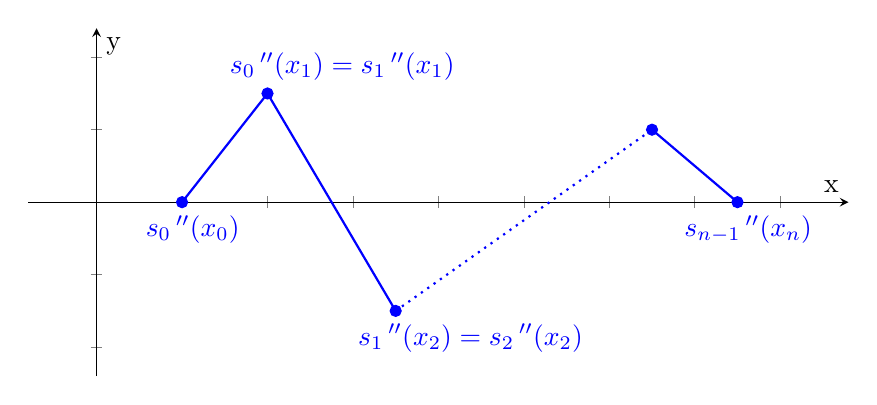
\begin{tikzpicture}

    \begin{axis}[
        legend pos=south east,
        axis x line=middle,
        axis y line=middle,
	xticklabels=\empty,
	yticklabels= \empty,
	%xtick={-1,-0.8,-0.6,-0.4,-0.2,0.2,0.4,0.6,0.8, 1},
	%ytick={0.25,0.5,0.75,1},
        grid = none ,
        width=12cm,
        height=6cm,
        grid style={dashed, gray!1},
        xmin=0,     % start the diagram at this x-coordinate
        xmax= 16,    % end   the diagram at this x-coordinate
        ymin=-4,     % start the diagram at this y-coordinate
        ymax= 4,   % end   the diagram at this y-coordinate
        %axis background/.style={fill=white},
        xlabel=x,
        ylabel=y,
        enlargelimits=true,
        tension=0.08]


  \addplot[blue, only marks, mark=*] coordinates {(2,0)(4,3)(7,-3)(13,2)(15,0)};
  \draw [blue,thick] (axis cs: 2,0) -- (axis cs: 4,3);
  \draw [blue,thick] (axis cs: 4,3) -- (axis cs: 7,-3);
  \draw [blue,thick,dotted] (axis cs: 7,-3) -- (axis cs: 13,2);
  \draw [blue,thick] (axis cs: 13,2) -- (axis cs: 15,0);
      

	\node(x0)[blue] at (axis cs: 2.25, -0.75){$s_0\,''(x_0)$};
	\node(x1)[blue] at (axis cs: 5.75,3.75){$s_0\,''(x_1)= s_1\,''(x_1)$};
	\node(x1)[blue] at (axis cs: 8.75,-3.75){$s_1\,''(x_2)= s_2\,''(x_2)$};
	\node(x0)[blue] at (axis cs: 15.25, -0.75){$s_{n-1}\,''(x_n)$};
    \end{axis}
\end{tikzpicture}
\end{document}